%IMPORTANT!!!!!! remember to abilitate twoside, openright to print document.
\documentclass[12pt]{report}%, twoside, openright]{report}
\usepackage[english]{babel}
\usepackage[utf8]{inputenc}
\usepackage{amsmath}
\usepackage{graphicx}
\graphicspath{{diagrams/}}
\usepackage{listings}
\usepackage{dirtytalk}

\usepackage[backend=biber,
						bibstyle=ieee,
						sorting = nty,
						citestyle=numeric-verb]{biblatex}
\bibliography{bibliography.bib}
\begin{document}

\begin{titlepage}

\newcommand{\HRule}{\rule{\linewidth}{0.5mm}}

\center % Center everything on the page

\textsc{\LARGE Fachhochschule Dortmund}\\[1.5cm] % Name of your university/college
\textsc{\Large Master Thesis for M. Eng. in Embedded Systems for Mechatronics}\\[0.5cm] % Major heading such as course name

\HRule \\[0.4cm]
{ \bfseries Development of a real-time software architecture for AMiRo robot based on the operator controller-module}\\[0.4cm] % Title of your document
\HRule \\[1.5cm]

\begin{minipage}{0.4\textwidth}
\begin{flushleft} \large
\emph{Author:}\\
Hector Gerardo Munoz Hernandez
\end{flushleft}
\end{minipage}
~
\begin{minipage}{0.4\textwidth}
\begin{flushright} \large
\emph{Supervisors:} \\
Prof. Dr. Carsten Wolff

Uwe Jahn
\end{flushright}
\end{minipage}\\[2cm]

{\large \today}\\[2cm]

\vfill
\end{titlepage}
\pagenumbering{roman}
\tableofcontents

\begin{abstract}
This work covers most of the internal controller required functionality assigned to the DA\_AMiRo project. The architecture of the AMiRo is briefly discussed and it is then explained how the three boards of the AMiRo talk to each other. Some other sensors are explained, and the Communication Area Network module. All these functionalities are incorporated in the sensor data handler which is explained later. Every piece of code described in the present report is part of the DA\_AMiRo project and the reader can go to the gitlab repository and the Wiki page for more information. One of the purposes of the DA\_AMiRo project is to compare its functionality with the DAEbot project conducted by Uwe Jahn. The reader can read all about the DAEbot's internal controller in the previous student's work \cite{DAEBot_internal}. This work will finalize with a comparison on both systems.
\end{abstract}
\pagenumbering{arabic}

\chapter{Introduction}
\section{Real-time Operating Systems}
The necessity to meet deadlines in today's projects is every time more demanded. Most applications consist of different tasks that can be executed in parallel, have different priority, have different period repetition, and frequently use shared resources. Using a multi-threading approach, however,  can create a challenge in terms of performance, stability and time of implementation.

An operating system is a software component of a computer system that is responsible for the management and coordination of activities and the sharing of the resources of the computer \cite{mcgraw}. "A real-time operating system perform these tasks, but is designed to run applications with a very precise timing and a high degree of reliability. This can be especially important in measurement and automation systems where downtime is costly or a program delay could cause a safety hazard" \cite{rtos}.

In other words, a real-time operating system is an operational system that provides certain capability according to preset timing constraints \cite{whatisRTOS}. This is achieved through a scheduler that is designed to provide a deterministic execution pattern. And so, the RTOS are used in systems with critical timing requirements, when each task should be executed within a restricted time interval \cite{whatisRTOS}.

When it can be guaranteed that a task will never exceed a maximum amount of time in being completed, it can be said that the operative system is "hard real-time". If it can be guaranteed that a task will most of the time not exceed a maximum amount of time in being completed, it can be said that the operative system is "soft real-time". An airbag system is an example of a "hard real-time" system, where the task has to be guaranteed to execute always within a time limit. For a "soft real-time" example, a video streaming can be considered, where an occasional loss of data can be accepted because it does not compromise the whole functionality \cite{rtos}.

In the real-time operating systems the managing of the tasks is crucial. To this end, programmers have to decide which task is running at certain time and how other tasks can preempt the processing resources if their priorities are higher. In other words, manage the schedule of the tasks so that they meet with their deadlines.

Some of the main characteristics of a RTOS are the following:

\begin{itemize}
\item Determinism: An application timing can be guaranteed within a certain margin of error.
\item Soft and Hard Real-Time: The validity of data after meeting a deadline. In soft real-time the deadline is not that crucial but in hard real-time the meeting of the deadline is very important.
\item Jitter: Which is the amount of error in the timing of a task over subsequent iterations of a program or loop \cite{whatisRTOS}.
\end{itemize}

\section{Operator Controller Module}

The DA\_AMiRo is inteded to work according to an OCM \cite{ocmAuto} software architecture similar to the one DAEbot was implemented with. In this structure there are three basic controllers: Internal Controller, Reflective Operator, and Cognitive Operator. In order to have a more precise overview of how these three controllers work in the DAEbot, figure \ref{fig:ocm} is explained by a direct quote from the Wiki:

\say{Refering to figure \ref{fig:ocm}, the Controllers (red) are used to connect all sensors and actuators. The Controllers need to be configured and programmed once, so the software on the controllers is mostly fixed and does not need to be flexible. The Reflective Operator(s) (yellow) control the Controllers. The Reflective Operator's software is the adaptable part of the distributed system - it changes from application to application. These Operator Controller Module(s) are located on the robot itself and let it act autonomously. The Cognitive Operator is hosted on a server and is used to optimize, program and interact with the user. The Cognitive Operator is connected via a wireless connection and can (only) interact with the Reflective Operator(s).}\cite{Wiki}.

\begin{figure}[h!t]
	\centering
	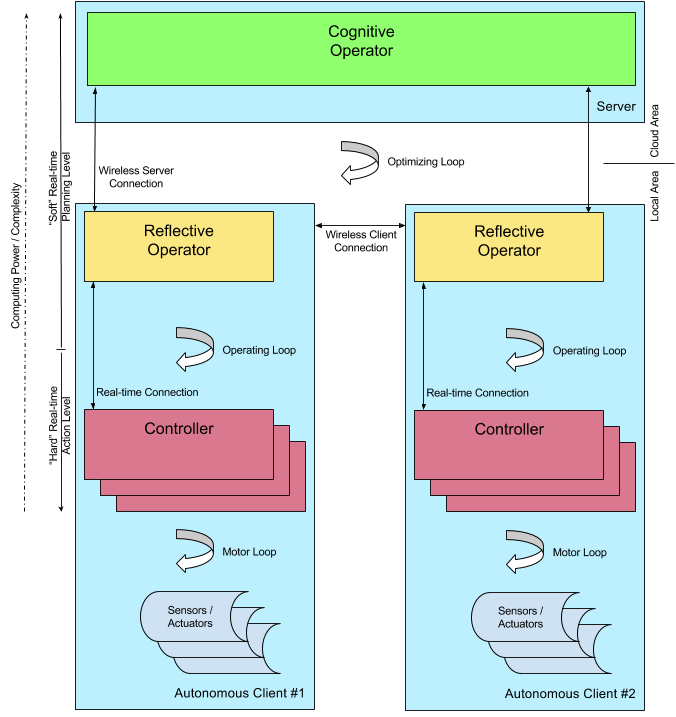
\includegraphics[width=\textwidth]{ocm}
    \caption{OCM software arquitecture for the DAEbot\cite{Wiki}.}
    \label{fig:ocm}
\end{figure}
\clearpage

The OCM was introduced by a group of Professors in the University of Paderborn. The concept aimed to structure and design a reconfigurable controller systems \cite{ocmAuto}. As mentioned before, there are three different levels in the OCM. The first one is the lowest level of the OCM also simply known as the Controller. This level interacts directly with the plant of the system, which means that the control signal is produced and measured here. It is also necessary that the software processing in this layer is quasi-continuous so that the measured values are processed in real-time conditions \cite{ocmAuto}.

The second layer is called the reflective operator. It is in this layer where the monitoring and the controlling routines are executed \cite{ocmAuto}. This layer does not have access to the actuators directly, because the Controller is already doing this. The expected result is that the Reflective Operator modifies the Controller, sometimes also changing between different pre-established Controller configurations. This level also requires a quasi-continuous operations like a continuous adaptation algorithm or a watchdog. This operator also has to operate under hard-time constraints because its relation with the Controller. In short, this layer serves as a interface between the Cognitive Operator and the Controller \cite{ocmAuto}.

The third layer is the Cognitive Operator. On this layer the system gathers information about itself and its environment to improve itself. This recollection of information can be done by applying various methods such as learning and model-based optimization among others. In other words, it is in this layer where the self-improvement takes place \cite{ocmAuto}.

This project focuses on the Controller and Reflective Operator of the AMiRo. The controller is the responsible for commanding the internal sensors of the STM32F32 boards inside AMiRo in real-time. This sensor information is then retrieved by the Reflective Operator with a demo application that will be explained later in this document inside section \ref{sect:example}.

\section{AMiRo}
The AMiRO project, which stand for Autonomous Mini Robot was started in the University of Bielefeld by Stefan Herbrechtsmeier and worked by Thomas Schöpping in collaboration with few others. The motivation for this project was to use small embedded systems in order to create a small robot that is easy to transport, usable on a table or the floor, appealing for young people, that is created with a modular approach is able to be extendable and customizable. With all of these aspects in mind, the result should be also a powerful tool for research and education \cite{AMiRo_ppt_v1}.

The preliminary work was conducted in the University of Paderborn in the form of the BeBot mini robot \cite{AMiRo_ppt_v1}. The intended architecture of both robots is a modular one, which means that it has more than one board functioning as a unity. In AMiRo's case, said architecture consisted on three boards, DiWheelDrive, Power Management, and Light Ring that will be discussed in the next chapter, and two main extension boards: the Cognition board and the Image Processing board. The former will be explained in section \ref{sub:cogn}, but the latter will not be discussed in this work, as it was not needed for the current reach of the project. If the reader is interested in the Image Processing board, he or she can refer to the project presentation given by Prof. Herbrechtsmeier \cite{AMiRo_ppt_v2}.

Physically AMiRo has a cylindrical shape with a diameter of 100mm. It is covered by a chassis that does not cover the DiWheelDrive board's bottom as this board has the proximity sensors pointing towards the ground. There are also two wheels with two separate motors directly connected to the DiWheelDrive board and two metal sliders for the robot stabilization in flat surfaces \cite{AMiRo_paper_modular}.

The chassis has three more openings for the following connections: USB serial that goes directly into the DiWheelDrive board, the power supply, and the charging pins. Additionally, when the Cognition board is attached, there are three more possibilities to physically interact with the robot: USB serial, USB dongle for wireless connection with the Linux OS, and a micro USB cable for connecting also with the Linux OS which is used in this board. The Cognition board will be later discussed in section \ref{sub:cogn}.

These characteristics make AMiRo a very compact and portable robot. Every board is designed to be modifiable, stackable and exchangeable with custom elements. All boards communicate with each other with the Controller Area Network protocol \cite{AMiRo_paper_modular}. This way every board can read any message from the CAN bus or write into it every time it is necessary.

\chapter{Architecture of AMiRo}
The AMiRo project was started in 2015 and ever since, the repository supporting the AMiRo project has had several updates \cite{AMiRo_Wiki}. It is worth mentioning that the version used as the basis for the present work was the version 1.0 stable. The AMiRo's repository consists of three basic folders: AMiRo bootloader, AMiRo Operating System, and ChibiOS.

Although this software architecture will be explained with more detail in section \ref{sec:soft}, it is worth mentioning that AMiRo's bootloader was used as it is in version 1.0 from the original repository in order to configure the computer for programming the AMiRo. The ChibiOS was also used as it is in version 1.0 from the repository \cite{AMiRo_Wiki}. The AMiRo Operating System was hugely modified to meet the requirements of the present work, which can be found under the current project's repository \textit{DA\_AMiRo} \cite{AMiRo_Git}.
%\footnote{AMiRo's original repository: https://openresearch.cit-ec.de/projects/amiro-os/wiki \cite{AMiRo_Wiki}}.

\section{Hardware Architecture of AMiRo}
As mentioned in the previous chapter, the AMiRo is equipped with three basic board modules and two extension boards. In this section each board will be briefly discussed with a special emphasis in the functionalities that are of interest for this work. For a more complete discussion about the boards or the AMiRo in general, the reader is invited to read the documentation referenced in this work, specially \cite{AMiRo_paper_verstaile, AMiRo_paper_modular, AMiRo_paper_applications, AMiRo_ppt_v1, AMiRo_ppt_v2} which can be found on the CITEC website or on the repository of this work on gitlab \cite{AMiRo_Git}.

The functionality of the sensors used in the project will be briefly explained in this chapter. For the explanation on how to read the output of the sensors that are sent via the Controller Area Network protocol, the reader is invited to jump directly into section \ref{sec:canconv} for reviewing the CAN convention used in the entire project and section \ref{sec:sensorout} for understanding each sensor's output.

\subsection{DiWheelDrive}
\label{sub:DWD}
The DiWheelDrive is the bottom board of the AMiRo. It is equipped with an ARM Cortex-M3 based STM32F103 MCU from STMicroelectronics \cite{AMiRo_paper_modular}. It is through the DiWheelDrive's UART interface that the AMiRo's three basic modules get programmed. Each board gets programmed at a time with help of the AMiRo bootloader which will be discussed in section \ref{sub:btl}.

This board has two motors of 1W DC. The purpose of having two motors was to be able to have a differential kinematic to allow flexible movements \cite{AMiRo_paper_modular}. Among other sensors and actuators, the ones that are in this board and are being used in this work are: three axis gyroscope, accelerometer, and magnetometer, floor proximity sensors, the two motors, and optical motor encoders. The functionality and some specifications of the above mentioned sensors and actuators will be discussed in the next subsections.

As mentioned before, the DiWheelDrive board has a Cortex-M3 MCU for calculating such things as motion control, odometry, and dead reckoning algorithms at high sampling rates \cite{AMiRo_paper_modular}. This board can be accessed by the other boards via the Controller Area Network protocol or via USB UART interface directly with the user. It is important to mention that every board has also a USB UART interface to communicate directly with the user but they are covered by the chassis except for the DiWheelDrive board \cite{AMiRo_paper_modular}.

\subsubsection{Gyroscope}
The gyroscope is a sensor that measures rotational motion. The units of the resulting measurement are revolutions per second or degrees per second. As a quick example, in a balancing robot a gyroscope can be used to measure how much the robot has rotated from the desired position and this information can be sent to an actuator to make corrections in order to reach the desired angle \cite{gyrostheory}. A gyroscope normally consists of a mass that moves with constant angular momentum, so when the gyroscope is tilted the axis of rotation of said mass reacts to the applied rotational movements making the axis of rotation tilt. This tilting leads to a displacement of the capacitance fingers inside the sensor which changes the capacitance. Finally when compared to a reference capacitance level, the angular velocity can be determined \cite{AMiRo_ppt_v1}.

The gyroscope used in the DiWheelDrive board is the l3g4200d from STMicroelectronics. This sensor communicates via SPI with the processor. This sensor is configured to have a resolution of $+/-500 dps$ in accordance with the user's manual \cite{gyroscopepart} and it is possible to obtain the output in degrees per second, micro degrees per second, revolutions per second, and micro revolutions per second with the actual code. The actual units are degrees per second but the user can easily change the output selecting a different function from \textit{updateSensorVal()} function inside DiWheelDrive.cpp. For a more clear explanation on the code structure, see section \ref{AMiRo_OS}. The sensor communicates with the processor via SPI communication.

\subsubsection{Accelerometer}
The accelerometer is a sensor that measures the acceleration of an object. The units of the resulting measurement are meters per squared second or in g forces, where g as a unit equals $9.81 m/s^2$ \cite{accelerometertheory}. It is typically a system composed by a mass, a spring, and a damper. The mass moves according to the applied acceleration and changes the resulting capacitance that can be sent as an output for further reading and processing \cite{AMiRo_ppt_v1}.

The accelerometer used in the DiWheelDrive board is the lis331dlh from STMicroelectronics. This sensor is configured be scaled with a $+/-8g$ factor in accordance with the user's manual \cite{accelerometerpart}. The output is in g units and the sensor is being communicated via SPI with the processor.

\subsubsection{Magnetometer}
The magnetometer is a sensor that measures the magnetic field for all three physical axes \cite{magnetometertheory}. This sensor works thanks to three principles. The first one is called the Anisotropic magneto resistance effect discovered in 1857 by William Thomson, in which an external magnetic field can make the sensor change the electrical resistance of a ferromagnetic material. The electrical resistance will be at a maximum value when the direction of the electrical current is parallel to said magnetic field \cite{AMiRo_ppt_v1}.

The second principle is called Fluxgate and it is a way of calculate the vectorial measurement of a magnetic field invented by Friedrich Förster in 1937. The method starts with two cores wrapped by two coils of wire. There should be an electrical current driving the core through cycles of magnetic saturation. The resulting electrical current of the second coil will depend on the external magnetic field \cite{AMiRo_ppt_v1}.

The last principle is called the Hall effect discovered in 1897 by Edwin Hall. In this principle can be visible when an electric current flows through a conductor in a magnetic field, the magnetic field will exert a transverse force on the moving charge carriers which tends to push them to one side of the conductor. The result is a voltage difference between both sides of the conductor \cite{halleffect}.

The magnetometer used in the DiWheelDrive board is the hmc5883l from STMicroelectronics. This sensor is configured to have a field resolution of $+/-5Gauss$ according to the user's manual \cite{magnetometerpart} and the current output is set to be in Gauss units. The sensor is being communicated via I2C protocol with the processor.

\subsubsection{Floor Proximity Sensor}
\label{sec:AMS}
The floor proximity sensor used is the "Fully Integrated Proximity and Ambient Light Sensor With Infrared Emitter", part vcnl4020 of Vishay \cite{proxsensor}. Four of these sensors are in the bottom of the AMiRo, programmed as light sensors, while other eight of these sensors are being used as proximity sensors and ambient light detectors coordinated by the Power Management board, see section \ref{PWB} for more information.

The ambient light sensor measures the intensity of light and its is measured in luminance. In order to do this the sensor usually consists of a photoresistor or a photo-sensitive material, outputting a resistance that can be measured and compared to a default value to estimate the luminance \cite{amstheory}.

The goal of providing AMiRo with these sensors attached to its bottom is to detect changes in the color of the floor. An example application can be for the AMiRo to follow a line or path painted on the ground, by making the robot recognize when it is over one color and when it is not.

\subsubsection{Motors}
As previously described in section \ref{sub:DWD}, the AMiRo has two DC motors of 1W each to offer a differential kinematic and to allow agile movements \cite{AMiRo_paper_modular}. These motors are connected to the DiWheelDrive board which means that this board controls the velocity of the motors and also knows the actual velocity of the motors.

The velocity of the motors can be set anytime from the Cognition board and the actual velocity of the AMiRo is one of the sensor values that can be asked from AMiRo's internal controller. The user can set and view the velocity in $\mu m/s$ or in $\mu rad/s$.

\subsubsection{Encoder}
AMiRo has optical encoders as well, that allow the user to know how much the motors have turned from a certain checkpoint. This data can be used to know how far the AMiRo has moved from a certain point. This sensor returns the $x$ coordinate in $\mu m$, the $y$ coordinate in $\mu m$, and the orientation of the wheels in $\mu rad$.

\subsection{Power Management}
\label{PWB}
The Power Management board is the central basic module of AMiRo. This board is responsible for the power supply and elementary behavior of the system. This is why it has the most powerful microcontroller. This board has an ARM Cortex-M4 based STM32F405 from STMicroelectronics. The characteristics from this microcontroller were needed to ensure a fast reaction times on critical system events and still provide enough headroom to additionally perform basic behaviors like obstacle avoidance, or homing \cite{AMiRo_paper_modular}.

There are two lithium-ion batteries connected to the Power Management board that power the whole system, and there are also some sensors on this board. Among the sensors that this board has, the ones that are being used by this project are: eight proximity sensors that act as proximity sensors and also as ambient light sensors, sensors for knowing if the charging cable is connected, the remaining battery charge or the time for a complete battery charge, the time for this both events to be completed, and the actual current consumption  \cite{AMiRo_paper_modular}.

\subsubsection{Power Status}
For the tracking of the power status, AMiRo is equipped with a bq27500 Impedance Track from Texas Instruments that allows the robot to obtain information such as remaining battery capacity, state-of-charge, run-time to empty, battery voltage, and temperature \cite{impedancepart}.

\subsubsection{Proximity Ring}
As seen in section \ref{sec:AMS}, the eight vcnl4020 sensors in connected to the Power Management board are functioning as ambient light sensors and also as proximity sensors. For this last functionality, the sensor has a built-in infrared emitter and photo-pin-diode, having a maximum relying measurement of 200mm \cite{proxsensor}. These sensors are connected in a ring-fashion way so that the AMiRo has eight sensors throughout its entire circumference, making it able to detect obstacles in all horizontal directions. The units of the output are also in mm.

\subsection{Light Ring}
The Light Ring board is the top-most board in the AMiRo. This board has a STMicroelectronics ARM Cortex-M3 based STM32F103 MCU. It contains eight RGB LEDs arranged in a circular way corresponding to the Proximity Ring discussed in last section. These LEDs can be set from the Cognition board, setting each color of the RGB channels \cite{AMiRo_paper_modular}.

\subsection{Cognition Board}
\label{sub:cogn}
This board was thought as an extension board which is no longer from the basic set of boards that make the AMiRo. The Cognition board in this project is being used as the Reflective Operator according to the OCM model. It provides all of the high-level tasks, gathering and coordinating the information generated in the three basic boards also known as the internal controller \cite{AMiRo_paper_modular}.

The most important feature of this board is the attached Gumstix Overo Computer-on-Module. In the current setup, the Overo TidalSTORM COM is being used, which combines an ARM Cortex-A8 based DaVinci DM3730 SoC from Texas Instruments \cite{AMiRo_paper_modular}. This board has the same serial programming port as on the three basic boards. It also has a Type A, a micro-AB, and an internal pin header USB interfaces \cite{AMiRo_paper_modular}.

The operating system running on the Overo COM is based on the Linux Yocto reference distribution Poky \cite{poky}, and the way it communicates with the three basic boards is through CAN, using a simple SocketCAN software-wrapper that is offered by this distribution \cite{AMiRo_paper_modular}.

\section{Software Architecture of AMiRo}
\label{sec:soft}
As it has been discussed in previous sections, the AMiRo project was started back in 2015 and it is still being maintained. The version 1.0 of the repository was the base used for this project \cite{AMiRo_Git}.

\subsection{AMiRo bootloader}
\label{sub:btl}
The open-source bootloader for MCUs is the bootstrap for the three basic boards of the AMiRo. The AMiRo's bootloader is the responsible of configuring and setting up the computer for working with the AMiRo. The set-up that is provided in the bootloader is more than enough to successfully start working on the Operating System of AMiRo and programming it \cite{btl}.

As said before, the DiWheelDrive is the only module of which the programming port can be accessed by the user. This is why new software is applied to the two other basic boards by remote flashing via OpenBLT. Using CAN communication the new binary is forwarded by the DiWheelDrive board so that the target board receives the data and stores it in its flash memory \cite{AMiRo_paper_modular}.

\subsection{AMiRo real-time operating system kernel}
For the real-time operating system the open-source ChibiOS was chosen. This project aims at creating a portable, light weight, and fast real-time operating system for embedded applications \cite{chibioshp}. ChibiOS not only provides low-level drivers for all interfaces of the most common microcontrollers, it also gives an unified hardware abstraction layer, priority based preemptive scheduling, and high-performance event and message passing systems. ChibiOS can be configured statically and dynamically to exactly fit the application in order to maximize efficiency and performance \cite{AMiRo_paper_modular}.

\subsubsection{ChibiOS}
Some of the main characteristics from ChibiOS are:

\begin{itemize}
\item System time: ChibiOS has a 16 or 32 bits system time counter.
\item Real tick-less mode: There is no periodic system tick for optimal power management.
\item IRQ Management: ISRs abstraction.
\item Preemption: Fully preemptive scheduling.
\item Round robin scheduling: Round robin scheduling for threads at equal priority.
\item Messages: Inter-thread synchronous messages.
\item Mailboxes: Message queues.
\item Counter semaphores: Semaphores with boolean state.
\item Binary semaphores: Semaphores with boolean state.
\item Mutexes: Mutexes implementing the priority inheritance algorithm.
\item Events: Events, event flags, event sources.
\item Dynamic services: Dynamic threading.
\end{itemize}
Note: All the above mentioned characteristics can be found and further explained in the ChibiOS homepage. \cite{chibioshp}

A project containing ChibiOS consists on the Operating System source files, few configuration files and a HAL file for the peripherals handling.

\subsection{AMiRo Operating System}
\label{AMiRo_OS}
AMiRo's Operating System or board specific abstraction layer from the original repository \cite{AMiRo_Wiki} includes two basic applications, the first one is a rudimentary command shell and the second one a hardware test. The first one is already integrated in ChibiOS and it is extended by module specific commands \cite{AMiRo_paper_modular}.

The structure of the AMiRo Operating System, including the files that are being used with the current project can be visualized in figure \ref{fig:OS}. The entire project is written in C++ language, with some inclusions of C code. In this figure, it can be seen that inside \textit{AMiRo\_OS} there is the \textit{components} folder which contains the shared codes that the three boards are using. The other part of the structure worth mentioning now is the \textit{devices} folder in which the three boards have their own set of files, always maintaining the same structure among them.

\begin{figure}[ht]
	\centering
	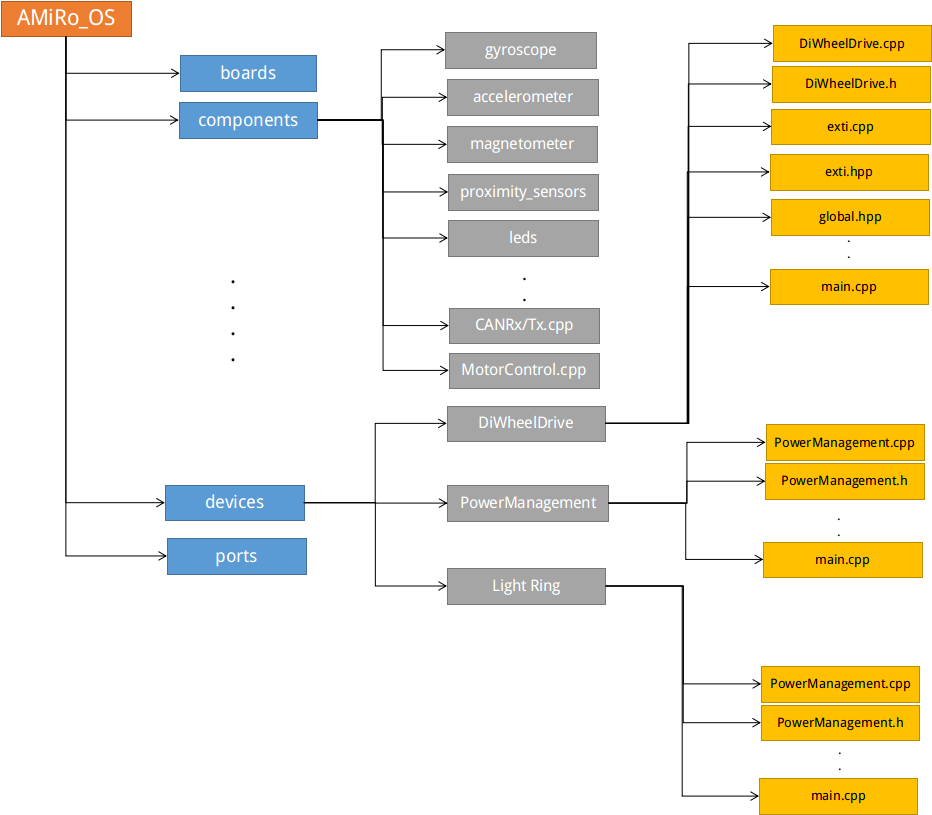
\includegraphics[width=\textwidth]{AMiRo_OS}
    \caption{AMiRo\_OS breakdown structure}
    \label{fig:OS}
\end{figure}

%Quizás algo más a cerca de AMiRo (apps, applicaciones pensadas, demos....)

\subsection{DA\_AMiRo software structure}
From the past sections the hardware and software structure of the AMiRo was mentioned and briefly discussed. From this point forward the structure and functionality of the DA\_AMiRo project will be discussed as it is the central point of the master thesis. As a friendly reminder, the reader can obtain the source codes made for the DA\_AMiRo project from the repository \cite{AMiRo_Git}.

In last section, the AMiRo's Operating System structure was introduced. This Operating System is the one located on top of figure \ref{fig:DAAMIROstr}, inside the folder called \textit{amiro\_1.0\_stable}. This Operating System was hugely modified to fit the requirements of the DA\_AMiRo project, and it's functionality will be discussed in section \ref{sub:DAAMIROOS}.

\begin{figure}[ht]
	\centering
	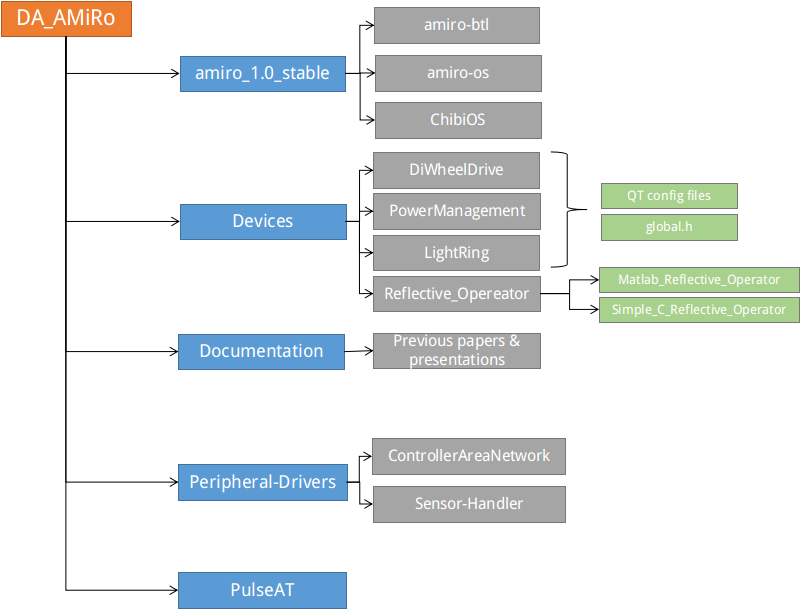
\includegraphics[width=\textwidth]{DAAMIRO}
    \caption{DA\_AMiRo overall structure}
    \label{fig:DAAMIROstr}
\end{figure}

The configuration files for the three projects are located inside the \textit{Devices} folder which can be visualized in figure \ref{fig:DAAMIROstr}. They configure the QT IDE for each of the three boards, so the user can easily code and create the binary to program the AMiRo's boards. It is also inside this folder where the Reflective Operator is located. The Reflective Operator consists of a simple C code for programming the MuRoX board, but also has a Matlab project responsible for creating an AMiRo's compatible program from a Simulink model. These issues will be discussed further in chapter \ref{chap:reflective}.

Inside the \textit{Peripheral-Drivers} the user can find the ControllerAreaNetwork.h responsible of having the structures and all the definitions that are being used by both the Internal Controller corresponding to the three basic boards and the Reflective Operator which is in charge of the MuRoX board. It is also inside this folder that the \textit{sensorhandler.cpp} and \textit{sensorhandler.h} are found. These both files manage the scheduling of the sensor data and they will be discussed in chapter \ref{chap:sensorDH}.

Finally, the folder \textit{Documentation} has some of the papers and information that the AMiRo has had since it was created. The reader can go inside this folder for getting more information about the AMiRo. In the other hand, the folder \textit{PusleAT} was created for a future reference and it is still a work in progress.

\subsection{DA\_AMiRo Operating System's functionality}
\label{sub:DAAMIROOS}
In this section, the functionality of the DA\_AMiRo Operating System from figure \ref{fig:OS} will be addressed.

The DiWheelDrive board, the DiWheelDrive class inherits from both ControllerAreaNetworkRx.cpp and from ControllerAreaNetworkTx.cpp, making it capable of sending and receiving CAN frames. This happens exactly the same in the three boards. The CAN frame structure will be further discussed in chapter \ref{chap:CAN}. The DiWheelDrive class also implements the functions for updating each of the sensor's values and sending independently the data via CAN interface. As it can be seen in figures \ref{fig:DWDclass}, \ref{fig:PMclass}, and \ref{fig:LRclass}, DiWheelDrive has virtual functions of every sensor including the Power Management board and also the Light Ring board. These functions however, have a '= 0' which means that they are not being implemented in this specific class. Similarly in the other two boards the same thing happens with their own set of sensors.

This means that in the DiWheelDrive class, the functions that are being implemented correspond to the gyroscope, accelerometer, magnetometer, proximity sensors, motors, and encoders. In the Power Management class the implemented functions include proximity sensors and power status sensors, and in the Light Ring class the implemented function concerns only the LEDs for the purposes of DA\_AMiRo.

The global class is the responsible for creating each object from each sensor and encapsulating them under the name of 'robot'. This makes the \textit{robot's} attributes accessible from other classes. This means that, for example, the gyroscope's value can be updated and outputted as a part of \textit{robot} from other parts of the code. The global object is finally initialized in the main function, as well as the threads responsible for managing the scheduler of the sensor's data but this subject will be discussed more deeply in chapter \ref{chap:sensorDH}.

\begin{figure}[ht]
	\centering
	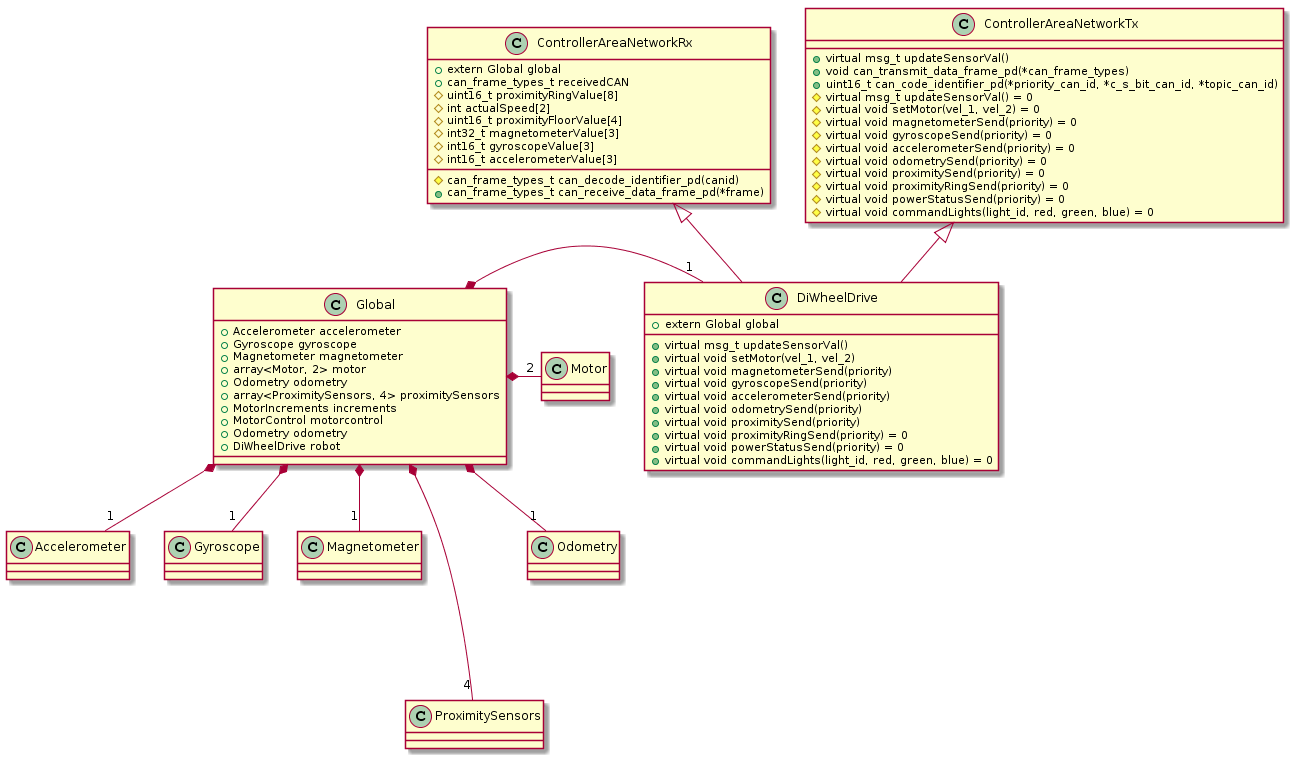
\includegraphics[width=\textwidth]{DWDclass}
    \caption{DiWheelDrive broad class diagram}
    \label{fig:DWDclass}
\end{figure}

\begin{figure}[ht]
	\centering
	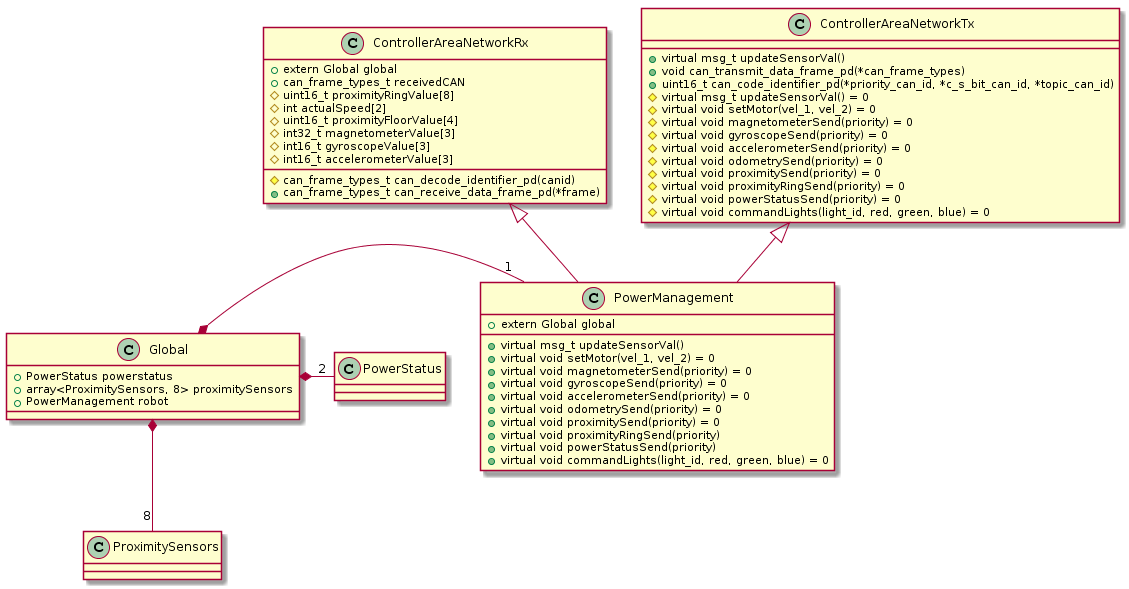
\includegraphics[width=\textwidth]{PMclass}
    \caption{PowerManagement broad class diagram}
    \label{fig:PMclass}
\end{figure}

\begin{figure}[ht]
	\centering
	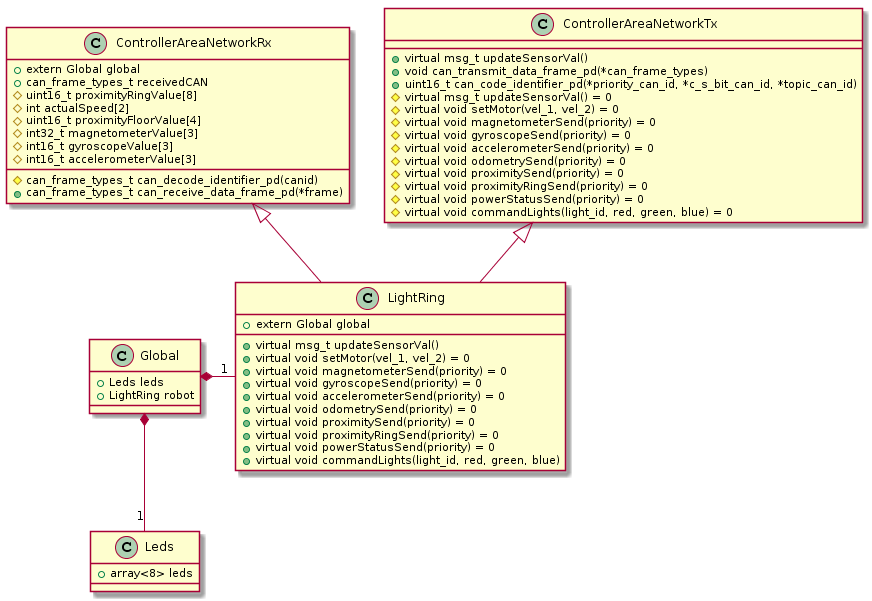
\includegraphics[width=\textwidth]{LRclass}
    \caption{LightRing broad class diagram}
    \label{fig:LRclass}
\end{figure}

\chapter{Controller Area Network}
\label{chap:CAN}
This chapter explains how to receive and transmit CAN frames in the AMiRo. The functionality of the CAN module had to be merged with the current ControllerAreaNetworkRx.cpp and ControllerAreaNetworkTx.cpp of the existing repository of AMiRo \cite{AMiRo_Wiki}. The ControllerAreaNetwork.h however, is the same that the DAEbot project is using. The reason behind sharing the ControllerAreaNetwork.h among projects is to be able to use a single Relfective Operator for both systems AMiRo and DAEbot so it is easier to compare functionalities.

\section{Convention used for sending and receiving frames}
\label{sec:canconv}

The format of the CAN frames was done accordingly with the pre-established convention for the DAEbot project \cite{DAEbot_Wiki}. The format of the standard id from a CAN frame can be seen in figure \ref{fig:can}, where it is basically divided into three main parts. The command or sensor bit is the bit that allows devices on the CAN bus to know if the frame belongs to a command, i.e. knowing the value 'x' axis of the gyroscope, or setting the LEDs to red, or if it belongs to a sensor frame, i.e. the actual value of the 'x' axis of the gyroscope.

The second part is the priority which allows the devices on the bus know the priority of the command or sensor. If there are two frames in the bus at the same time asking for a sensor value from the same board for example, the priority will allow the system to preempt the frame of the one with higher priority.

The third and last part of the id from the frame is the topic id. The list for the topics can be seen in the ControllerAreaNetwork.h shared by all the devices or also from the ods file inside the same path \textit{Peripheral-Drivers/ControllerAreaNetwork/} from figure \ref{fig:DAAMIROstr}.

\begin{figure}[ht]
	\centering
	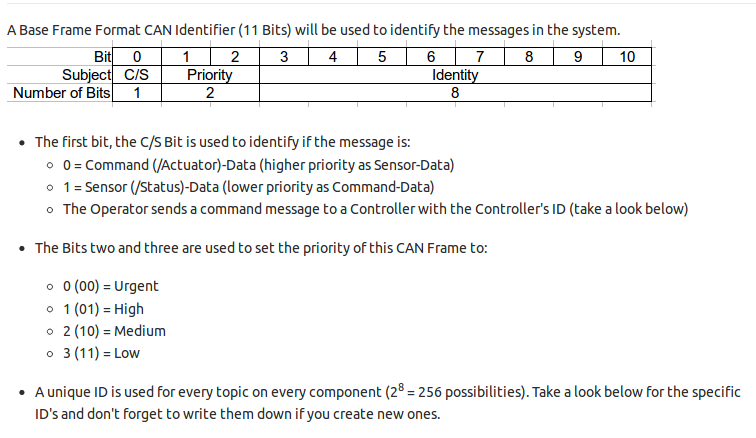
\includegraphics[width=\textwidth]{can_structure}
    \caption{Pre-established CAN frame format \cite{DAEbot_Wiki}}
    \label{fig:can}
\end{figure}

For the transmission of a CAN frame, the id is coded according to figure \ref{fig:can} and when a CAN frame is received, the id is decoded into the same structure. The CAN frame pre-established structure can be seen in snip of code \ref{CAN:frame}, which can be compared with the figure \ref{fig:can}. In this structure the only thing that has not been yet discussed is the data itself. The dlc is the number of bytes to be transmitted and the information is stored in the data8, data16 and data32 arrays. Thanks to the \textit{union} of these arrays, the same value can be accessed in different bit sizes.

\begin{minipage}{\linewidth}
\begin{lstlisting}[caption = CAN frame, label = CAN:frame, language = C, captionpos = b]
typedef struct can_frame_types {
    priority_can_id_t priority_id;
    c_s_bit_can_id_t c_s_bit_id;
    topic_can_id_t topic_id;
    uint8_t dlc;
    union{
        uint8_t     data8[8];
        uint16_t    data16[4];
        uint32_t    data32[2];
    };
} can_frame_types_t;
\end{lstlisting}
\end{minipage}

In order to send a CAN frame, can\_transmit\_data\_frame\_pd(...) can be called. When sending a CAN frame, the id is set to be in standard mode. The CAN frame that is sent consists of three main parts: id, DLC, and the data. The id is therefore set with the can\_code\_identifier\_pd(...) function before actually calling the transmit function. This function combines the c\_s bit with the priority bit and then combines that value to the topic ID. The CAN frame is later sent through the CAN driver.

On the CAN reception side, the status of the reception is assigned when calling to the can\_receive\_data\_frame\_pd(...) function. The status of the CAN reception can be successful, timeout, or error. Then the id of the CAN frame gets decoded with the function can\_decode\_identifier\_pd(...) and the data frames are passed into a global structure like in snip of code \ref{CAN:frame}

Note that can\_code\_identifier\_pd(...) and can\_decode\_identifier\_pd(...) are functions that were already implemented beforehand, for this project it was necessary to adjust both functions to operate with the current hardware platform.

\section{Interpreting CAN frames of the sensors}
\label{sec:sensorout}
In this section it will be explained how to read the frames corresponding to each sensor. For the same reason, this section is divided into two subsections: sensors and actuators.

\subsection{Sensors}
In order to interact with a sensor, the id from the CAN frame's command has to obey the convention shown in figure \ref{fig:can} and its content, the actual data from the CAN frame has to follow the convention shown in figure  \ref{fig:sensormodes} created by Uwe Jahn for the DAEbot project.

There are three ways or modes in which a command can ask for data from a sensor. The first one is the mode one which asks for a sensor's data with a specific frequency. The first DLC of the CAN frame has to be set to '1' to activate the publisher mode. The second and third DLCs specify the numeric value of the frequency in format of little-endian. This means that the most significant bit should be a part of the DLC number 2 and the less significant bit should be a part of the DLC number 1. The fourth DLC specify the units of the value given in the second and third DLCs. This value can be obtained looking at figure \ref{fig:sensormodes}.

\begin{figure}[ht]
	\centering
	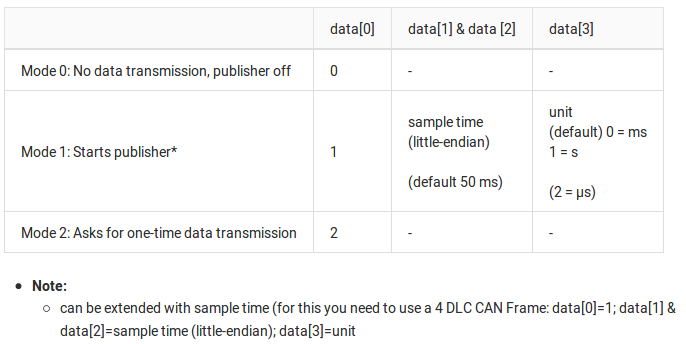
\includegraphics[width=\textwidth]{modes}
    \caption{Pre-established CAN modes for transmitting sensor data \cite{DAEbot_Wiki}}
    \label{fig:sensormodes}
\end{figure}

For example for starting publisher of the magnetometer 'x' axis, with normal priority, the CAN id should be composed by:
\begin{itemize}
	\item C\_S bit set to '0' on binary
	\item Priority set to '10' on binary
	\item Topic id of the gyroscope 'x' axis '0x05' on hexadecimal
\end{itemize}

So a value equal of '01000000101' in binary or '0x205' in hexadecimal. Now lets say we want the magnetometer 'x' axis value every $900\mu s$. The value '900' in decimal is '0x0384' in hexadecimal, making the little-endian adjustment for the bytes will result in '8403'. $\mu s$ is equal to '0x02'.

As a result, the complete CAN frame is: '0x205' for the id, '4' for the DLC or Data Length Code, each with the following values:

\begin{itemize}
	\item DLC 0: 0x01
	\item DLC 1: 0x84
	\item DLC 2: 0x03
	\item DLC 3: 0x02
\end{itemize}

This command would trigger the DiWheelDrive to output the magnetometer 'x' axis value every $900\mu s$, with an id that is almost the same but with the C\_S bit set to '1' instead, so that the CAN bus knows that this frame belongs to a sensor data. The topic id then will be '0x605' instead of '0x205'. The way of reading and understanding the outputted value for each sensor will be mentioned in the following subsections.

The second mode is the \textit{One-time data transmission} and it will only return the required sensor value one time. For the example of a one time transmission of the floor proximity sensors, the id of the CAN frame should be '0x204' with DLC 0: 2.

The third mode is the mode '0' which actually stops an on-going publishing of a sensor value given the frame's id. This means that in the example used for the explanation of mode '1' the way of stopping the transmission of the magnetometer 'x' axis, the id of the CAN frame should be the same '0x205', with DLC 0: 0.

\subsubsection{Gyroscope}
The three axis of the gyroscope come together in one CAN frame with a DLC of six. Each value has a size of 16bits with a format  of little-endian. Every value comes in two's complement and the units are degrees per second, and the resolution is $+/-500 dps$. See table \ref{tab:gyroscope}.

\begin{table}[h!]
\centering
\begin{tabular}{|l|l|}
	\hline
	DLC						&	6													\\	\hline
	size of data	&	16bits										\\	\hline
	'x' axis			&	DLC[1] DLC[0]							\\	\hline
	'y'	axis			&	DLC[3] DLC[2]							\\	\hline
	'z'	axis			&	DLC[5] DLC[4]							\\	\hline
	units					&	dps												\\	\hline
	note					& value in two's complement \\	\hline
\end{tabular}
\caption{\label{tab:gyroscope} CAN frame format from the output of the gyroscope}
\end{table}

\subsubsection{Accelerometer}
The three axis of the accelerometer come together in one CAN frame with a DLC of six as the gyroscope. Each value has a size of 16bits with a format of little-endian. Every value comes in two's complement and the units are $g$, and the result is scaled $+/-8g$. See table \ref{tab:accelerometer}.

\begin{table}[h!]
\centering
\begin{tabular}{|l|l|}
	\hline
	DLC						&	6													\\	\hline
	size of data	&	16bits										\\	\hline
	'x' axis			&	DLC[1] DLC[0]							\\	\hline
	'y'	axis			&	DLC[3] DLC[2]							\\	\hline
	'z'	axis			&	DLC[5] DLC[4]							\\	\hline
	units					&	g													\\	\hline
	note					& value in two's complement \\	\hline
\end{tabular}
\caption{\label{tab:accelerometer} CAN frame format from the output of the accelerometer}
\end{table}

\subsubsection{Magnetometer}
In the case of the Magnetometer, every axis has an independent id, this is because the size of the data is 32bits in little-endian format. Every value comes in two's complement and the units are $Gauss$, and the result is scaled by $+/-5Gauss$. See table \ref{tab:magnetometer}.

\begin{table}[h!]
\centering
\begin{tabular}{|l|l|}
	\hline
	DLC						&	4														\\	\hline
	size of data	&	32bits											\\	\hline
	'x' axis			&	DLC[3] DLC[2] DLC[1] DLC[0]	\\	\hline
	'y'	axis			&	DLC[3] DLC[2] DLC[1] DLC[0]	\\	\hline
	'z'	axis			&	DLC[3] DLC[2] DLC[1] DLC[0]	\\	\hline
	units					&	Gauss												\\	\hline
	note					& value in two's complement 	\\	\hline
\end{tabular}
\caption{\label{tab:magnetometer} CAN frame format from the output of the magnetometer}
\end{table}

\subsubsection{Floor proximity sensors}
The four proximity sensors on the bottom of the AMiRo are together in one CAN frame with a DLC of eight. Each value has a size of 16bits with a format of little-endian. The data is in luminance with units candelas per squared meter $cd/m^2$. See table \ref{tab:floorprox} and note that this sensor does not return a two's complement value.

\begin{table}[h!]
\centering
\begin{tabular}{|l|l|}
	\hline
	DLC						&	8													\\	\hline
	size of data	&	16bits										\\	\hline
	sensor 1			&	DLC[1] DLC[0]							\\	\hline
  sensor 2			&	DLC[3] DLC[2]							\\	\hline
	sensor 3			&	DLC[5] DLC[4]							\\	\hline
	sensor 4			&	DLC[7] DLC[6]							\\	\hline
	units					&	$cd/m^2$									\\	\hline
\end{tabular}
\caption{\label{tab:floorprox} CAN frame format from the output of the floor proximity sensors}
\end{table}

\subsubsection{Encoder}
This sensor returns the 'x' coordinate in $\mu m$ with a size of 32bits, the 'y' coordinate in $\mu m$ with a size of 32bits, and the orientation of the wheels in $\mu rad$ with a size of 16bits. All of these values are together in one CAN frame. See table \ref{tab:encoder}.

\begin{table}[h!]
\centering
\begin{tabular}{|l|l|}
	\hline
	DLC										&	8																\\	\hline
	size of data					&	32 bits, 32 bits, and 16 bits		\\	\hline
	'x' coordinate				&	DLC[0] DLC[1] DLC[2] 						\\	\hline
	'y'	coordinate				&	DLC[3] DLC[4] DLC[5] 						\\	\hline
	orientation of wheels	&	DLC[6] DLC[7] 									\\	\hline
	units									&	$\mu m$, $\mu m$, and $\mu rad$	\\	\hline
\end{tabular}
\caption{\label{tab:encoder} CAN frame format from the encoder}
\end{table}

\subsubsection{Actual velocity}
This id returns the 'x' velocity in $\mu m/s$ with a size of 32bits and the 'z' angular velocity in $\mu rad/s$ also in 32bits. These two values are together in one CAN frame. See table \ref{tab:velocity}.

\begin{table}[h!]
\centering
\begin{tabular}{|l|l|}
	\hline
	DLC										&	8														\\	\hline
	size of data					&	32bits											\\	\hline
	'x' velocity					&	DLC[0] DLC[1] DLC[2] DLC[3]	\\	\hline
	'z'	angular velocity	&	DLC[4] DLC[5] DLC[6] DLC[7]	\\	\hline
	units									&	$\mu m/s$ and $\mu rad/s$		\\	\hline
\end{tabular}
\caption{\label{tab:velocity} CAN frame format from the output of the actual velocity}
\end{table}

\subsubsection{Power Status}
When the id for the power status is asked, four values are sent within one CAN frame. The charging or no charging flag in 8bits, the state of charge in percentage in 8bits, the minutes remaining for a complete charge when the flag for charging is 'on' and the minutes remaining of battery power when the flag for charging is 'off' in 16bits and in little-endian, and the current power consumption in $mW$ also in 16 bits and in little-endian. See table \ref{tab:powerstatus}.

\begin{table}[h!]
\centering
\begin{tabular}{|l|l|l|}
	\hline
	DLC										&	6																	&																					\\	\hline
	size of data					&	8bits, 8bits, 16bits, and 16bits	&																					\\	\hline
	charging flag					&	DLC[0]														& '0' for not charging, '1' for charging	\\	\hline
	state of charge				&	DLC[1] 														&	percentage															\\	\hline
	time until charge			&	DLC[3] DLC[2] 										&																					\\	\hline
	time until charge			&	DLC[5] DLC[4] 										&																					\\	\hline
	units									&	percentage, minutes, $mW$					&																					\\	\hline
\end{tabular}
\caption{\label{tab:powerstatus} CAN frame format from the output of the power status}
\end{table}

\subsubsection{Proximity ring}
The proximity ring will return eight CAN frames one for every sensor there is. Each value is of 16btis and it is in little-endian, and the units are $mm$. See table \ref{tab:proxring}.

\begin{table}[h!]
\centering
\begin{tabular}{|l|l|}
	\hline
	DLC						&	16												\\	\hline
	size of data	&	16bits										\\	\hline
	sensor 1			&	DLC[1] DLC[0]							\\	\hline
  sensor 2			&	DLC[1] DLC[0]							\\	\hline
	sensor 3			&	DLC[1] DLC[0]							\\	\hline
	sensor 4			&	DLC[1] DLC[0]							\\	\hline
	sensor 5			&	DLC[1] DLC[0]							\\	\hline
  sensor 6			&	DLC[1] DLC[0]							\\	\hline
	sensor 7			&	DLC[1] DLC[0]							\\	\hline
	sensor 8			&	DLC[1] DLC[0]							\\	\hline
	units					&	$mm$											\\	\hline
\end{tabular}
\caption{\label{tab:proxring} CAN frame format from the output of the proximity ring sensors}
\end{table}

\subsection{Actuators}
There are so far two implemented actuators: the motors and the LEDs. The way of interacting with the sensors will be now described but it is important to note that they will not send anything back to the CAN bus, as they will only 'act'.

\subsubsection{Motors}
For the motors, the

\subsubsection{LEDs}


\chapter{Sensor data handler}
\label{chap:sensorDH}

\section{Overall functionality}

\section{Implementing modes}

\section{Real-time implementation}
%al final decir que funciona ya independientemente como un sólo internal controller.

\chapter{MuRoX board}
\label{chap:reflective}

\section{Compiling for MuRoX}

\section{Example application}
\label{sect:example}

\section{Compiling from Simulink for MuRoX}

\chapter{Results}
\section{AMiRo vs. DAEbot}

\section{Outlook}

%bibliography
\printbibliography
\nocite{*}

\end{document}
\grid
